Consider an ellipse $\mathcal{E}=\{p\in \mathbb{R}^2:  \langle Ap,p\rangle=1\}$, where  $A$ is a positive  self-adjoint matrix.

In an elliptic billiard orbit $ (x_k,y_k)$ with $x_k\in\mathcal{E}$ and a unit vector $y_k\in \mathbb{R}^2$ we have that:
\begin{align*}
	x_{k+1} &=x_k\;+\mu_k y_{k+1},\;\;\;\;
	y_{k+1} =y_k+\; \nu_k Ax_{k}\\
	\nu_k &=\;-\frac{2\langle Ax_k,y_k\rangle}{\langle Ax_{k},Ay_{k}\rangle},\;\;\;\;
	\mu_k  =\;-\frac{2\langle Ay_{k+1},x_k\rangle}{\langle Ay_{k+1},y_{k+1}\rangle},\;\;\;
	y_{k+1}  =\;\frac{x_{k+1}-x_k}{|x_{k+1}-x_k|}
\end{align*}
\begin{figure} 
\begin{center}
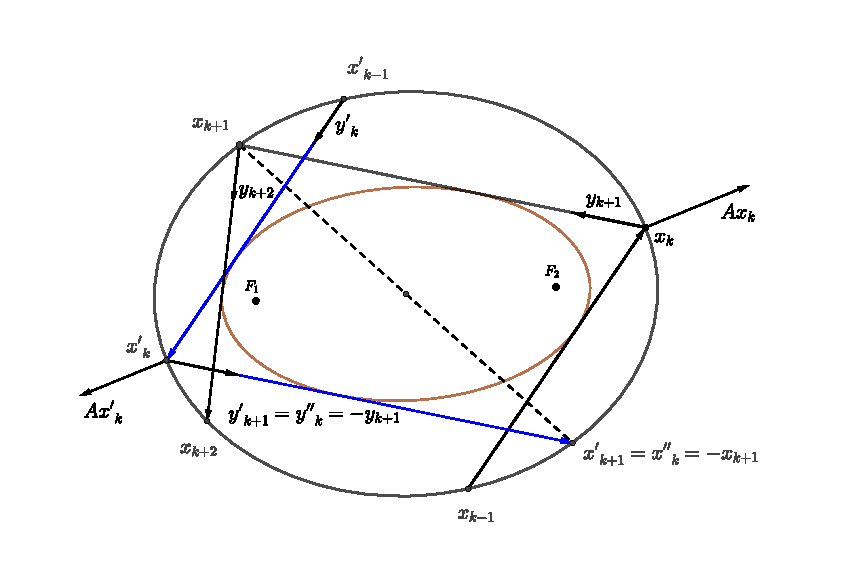
\includegraphics[scale=0.8]{pics_09_030_veselov2.pdf}
\caption{The skew-hodograph map $\phi(x_k,y_k)=(x'_k,y'_k)$ commutes with $T$ and $\phi^2=-T$.}
\end{center}
\end{figure}
   
 
 

Let the skew-hodograph mapping $\phi(x,y)=(x',y')$ defined by

\begin{align}
    x'_k&=Cy_{k+1}=C(y_k+\nu_k Ax_k)\nonumber \\
    y'_k&=-C^{-1}x_k, \;\; C=A^{-\frac{1}{2}}
    \label{eq:hodrog}
\end{align}

\begin{proposition}
    \label{prop:veselov}
    Let $T(x_k,y_{k})=(x_{k+1},y_{k+1})$ the billiard map.
    Then $\phi\circ T=T\circ \phi$ and $\phi^2=\phi\circ\phi=-T.$
\end{proposition}
\begin{proof} Since $A $ and $C$ are selfadjoint matrices it follows that:
 
\begin{align*}
    \langle A x'_k,x'_k\rangle & =\langle A  Cy_{k+1},Cy_{k+1}\rangle= \langle A  A^{-\frac{1}{2} }y_{k+1},A^{-\frac{1}{2} }y_{k+1}\rangle=\langle A^{\frac{1}{2}  } y_{k+1},A^{-\frac{1}{2} } y_{k+1}\rangle\\
    &=\langle A^{-\frac{1}{2} }A^{ \frac{1}{2} } y_{k+1} ,  y_{k+1}\rangle=\langle y_{k+1} ,  y_{k+1}\rangle=1\\
   \langle y'_k,y'_k\rangle & = \langle -C^{-1}  x_{k},-C^{-1}x_{k}\rangle   = \langle A^{\frac{1}{2}}  x_{k },A^{\frac{1}{2} } x_{k }\rangle = \langle A   x_{k },  x_{k }\rangle=1.
\end{align*}
Straightforward calculations shows that
\[ \nu'_k=-\mu_k, \;\; \mu'_k=-\nu_{k+1}.\]

\noindent Therefore,
\begin{align*}
     x'_{k+1}-x'_k&=C(y_{k+2}-y_{k+1})=C\nu_{k+1}Ax_{k+1}=\nu_{k+1}A^{\frac{1}{2}}x_{k+1}\\
     &=-\nu_{k+1}C^{-1} x_{k+1} 
    = -\nu_{k+1} y'_{k+1}
     =\mu'_ky'_{k+1}\\ y'_{k+1}-y'_k&=-C^{-1}(x_{k+1}-x_k)=-C^{-1}(\mu_ky_{k+1})=-\mu_kC^{-1}(C^{-1} x'_k)\\
     &=-\mu_k A^{\frac{1}{2}}A^{\frac{1}{2}} x'_k=-\mu_kAx'_k=\nu'_kA x'_k. \end{align*}
This means that the $(x'_k,y'_k)$ is also a billiard orbit and so
 $\phi\circ T= T\circ \phi.$
Finally,
\begin{align*}
    x''_k&=Cy'_{k+1}=C(-C^{-1} x_{k+1})=-x_{k+1}\\
    y''_k&=-C^{-1}x'_k=-C^{-1}(Cy_{k+1})=-y_{k+1}
\end{align*}
So, $\phi^2=-T.$
\end{proof}